\chapter{Инциденты на АЭС в Испании}

Инцидентам на АЭС принято присваивать рейтинг опасности в соответствии с Международной шкалой ядерных событий. Данная шкала была разработана в 1988 году и с этого момента использовалась в целях единообразия оценки чрезвычайных случаев, связанных с аварийными радиационными выбросами в окружающую среду на атомных станциях. Графическое изображение приведено на рисунке \ref{pic:INESscale}.

Как можно видеть нулевой уровень присваивается чему-либо не несущему какого-либо вреда, незначительным происшествиям соответствуют уровни от 1 до 3, серьезные же инциденты имеют уровни от 4 до 7.

\begin{figure}[h]
	\begin{center}
		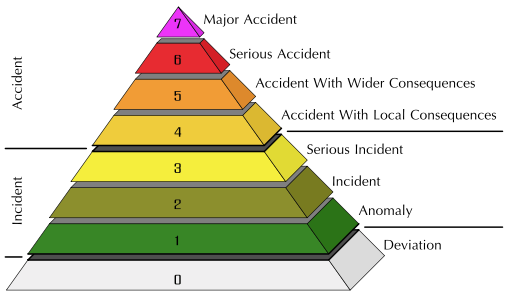
\includegraphics[width=.5\columnwidth]{./img/INESscale.png}
	\end{center}
	\caption{Международная шкала ядерных событий}
	\label{pic:INESscale}
\end{figure}

За историю атомной энергетики Испании инциденты происходили на 3-ех атомных электростанциях - АЭС Вандельос, АЭС Аско и АЭС Альмарас.
Следуя в хронологическом порядке, в 1989 году произошел инцидент на одной из первой АЭС страны - Вандельос.

В турбинном отделении Блока 1 19 октября 1989 года произошло возгорание, впоследствии согласно шкале INES данному случаю был присвоен 3-ий уровень (серьезный инцидент), однако никаких выбросов, вредных для окружающей среды зафиксировано не было.
Началом инцидента послужило уничтожение одной из лопаток энергогенерирующей турбины. Следствием этого стало возгорание турбинного масла и водорода, которое служило охлаждением для турбины. Быстрое распространение огня привело к уничтожению электропроводки как в системах нормальной эксплуатации, так и в аварийных системах. Результатом стало повреждение многих систем отвечающих за безопасность и отвод остаточного тепловыделения. Однако, эффективные действия, предпринятые сотрудниками, находившимися на станции, по использованию минимального количества средств обеспечения безопасности, спасли реактор от перегрева и повреждения ядерного топлива \cite{nuclearSafety}.

Согласно \cite{sympaperRodriguez} этот инцидент оказал значительное влияние на практики проектирование пожарозащиты на АЭС по всему миру. Тем не менее, несмотря на то, что последствия удалось устранить было принято решение о выводе из эксплуатации Блока 1. В период с 1990 по 1997 год осуществлялась полная выгрузка со станции ядерного топлива, переработка отходов АЭС. Затем, в период с 1998 по 2003 год были отключены большинство сооружений энергоблока. В изначальном состоянии осталась внутренняя часть реактора и фундамент, работы по их демонтажу планируется провести через 30 лет, когда радиационная активность уменьшиться достаточно, чтобы сделать работы максимально простыми.

Инцидент имел большое влияние на проектировщиков АЭС во всём мире, извлёкших многочисленные уроки из этого события, что привело к пересмотру многих вопросов пожарозащиты станций. Также инцидент оказал серьёзное негативное влияние на общественное мнение в Испании в сфере строительства АЭС \cite{sympaperRodriguez}.

Следующим инцидентом на АЭС Вандельос стала течь в трубопроводе из-за коррозии. Инцидент произошел 25 августа 2004 года на Блоке 2. В результате течи блок пришлось остановить согласно регламенту. Инцидент получил уровен 2 по шкале INES. По результатам инцидента была переработана система технического водоснабжения \cite{nuclearRegulatory}.

Менее серьезный, но все же инцидент произошел на АЭС Альмарас в мае 2003 года - было зафиксировано, что один из реакторов станции перегревался, в связи с чем он был остановлен на два с лишним месяца. В результате, испанские специалисты не смогли решить проблему и задачу пришлось отдать на исполнение французской компании \cite{miraesAlmaras}

Последней АЭС, об инцидентах на которой известно является АЭС Аско. Первый инцидент произошел в ноябре 2007 года на реакторе первого блока. Происшествием стал выброс радиации при загрузке топлива, классифицирован 2-ым уровнем опасности. О ней стало известно лишь в марте 2008 в результате обнаружения повышенной радиоактивности в воздухе вокруг АЭС. В результате инцидента был уволен директор станции и была заражена радиацией свалка, на которую вывозился мусор со станции \cite{miraesAsko}.

Позже, в сентябре 2008 из-за утечки масла из одного из агрегатов блок Аско-1 был остановлен. 20 июля 2009 года Аско-1 была повторно остановлена в виду самопроизвольной активации двух из четырех каналов для измерения потока нейтронов \cite{aesAsko}.